\chapter{Sprint 03 – Gestion des ordres de mission}
\section*{Introduction}

Ce sprint est consacré à l’implémentation du module de gestion des ordres de mission, qui constitue le cœur opérationnel de la plateforme. Il permet de gérer le cycle de vie complet d’une mission, depuis la demande exprimée par un client jusqu’à sa réalisation par un prestataire, en passant par l’attribution, le suivi et la facturation.

L’objectif principal de ce sprint est de structurer les interactions entre clients et prestataires autour des ordres de mission, tout en assurant une traçabilité claire et une logique métier cohérente.

Les fonctionnalités mises en œuvre incluent :
\begin{itemize}
  \item La consultation par les prestataires des ordres de mission disponibles ;
  \item La possibilité pour un prestataire d’exprimer son intérêt pour une mission ;
  \item Le suivi des missions confirmées dans l’agenda du prestataire ;
  \item La génération automatique de la facture à la fin d’une mission.
\end{itemize}

Ce sprint assure ainsi la fluidité du processus de mise en relation et de réalisation de service au sein de la plateforme.


\section{Sprint 03 Backlog – Gestion des ordres de mission}

\begin{table}[H]
\centering

\begin{tabular}{|c|p{4.2cm}|c|p{5cm}|c|c|}
\hline
\textbf{ID US} & \textbf{User Story} & \textbf{ID Task} & \textbf{Task} & \textbf{Estimation} & \textbf{Responsable} \\
\hline

US03-01 & En tant que prestataire, je peux consulter les ordres de mission disponibles.
     & US03-01.1 & Créer l’API de récupération des ordres & 2h & Aziz \\
     \cline{3-6}
     & & US03-01.2 & Afficher les ordres dans Angular & 2h & Aziz \\
\hline

US03-02 & En tant que prestataire, je peux exprimer mon intérêt pour une mission. 
     & US03-02.1 & Ajouter bouton “Exprimer intérêt” dans Angular & 1h30 & Aziz \\
     \cline{3-6}
     & & US03-02.2 & Mettre à jour le backend pour enregistrer l’intérêt & 1h30 & Aziz \\
\hline

US03-03 & En tant que prestataire, je peux suivre les missions confirmées. 
     & US03-03.1 & Créer endpoint GET /orders/confirmed & 1h30 & Aziz \\
     \cline{3-6}
     & & US03-03.2 & Afficher dans la vue “My Work” & 2h & Aziz \\
\hline

US03-04 & En tant que prestataire, je peux générer une facture après la mission. 
     & US03-04.1 & Développer le calcul de rémunération + génération facture & 2h & Aziz \\
     \cline{3-6}
     & & US03-04.2 & Afficher la facture générée dans l’interface Angular & 1h30 & Aziz \\
\hline

\end{tabular}
\caption{Product Backlog – Sprint 03 : Gestion des ordres de mission}
\label{tab:product_backlog_orders}
\end{table}


\section*{Diagramme de cas d'utilisation}
    \begin{figure}[H]
    \centering
    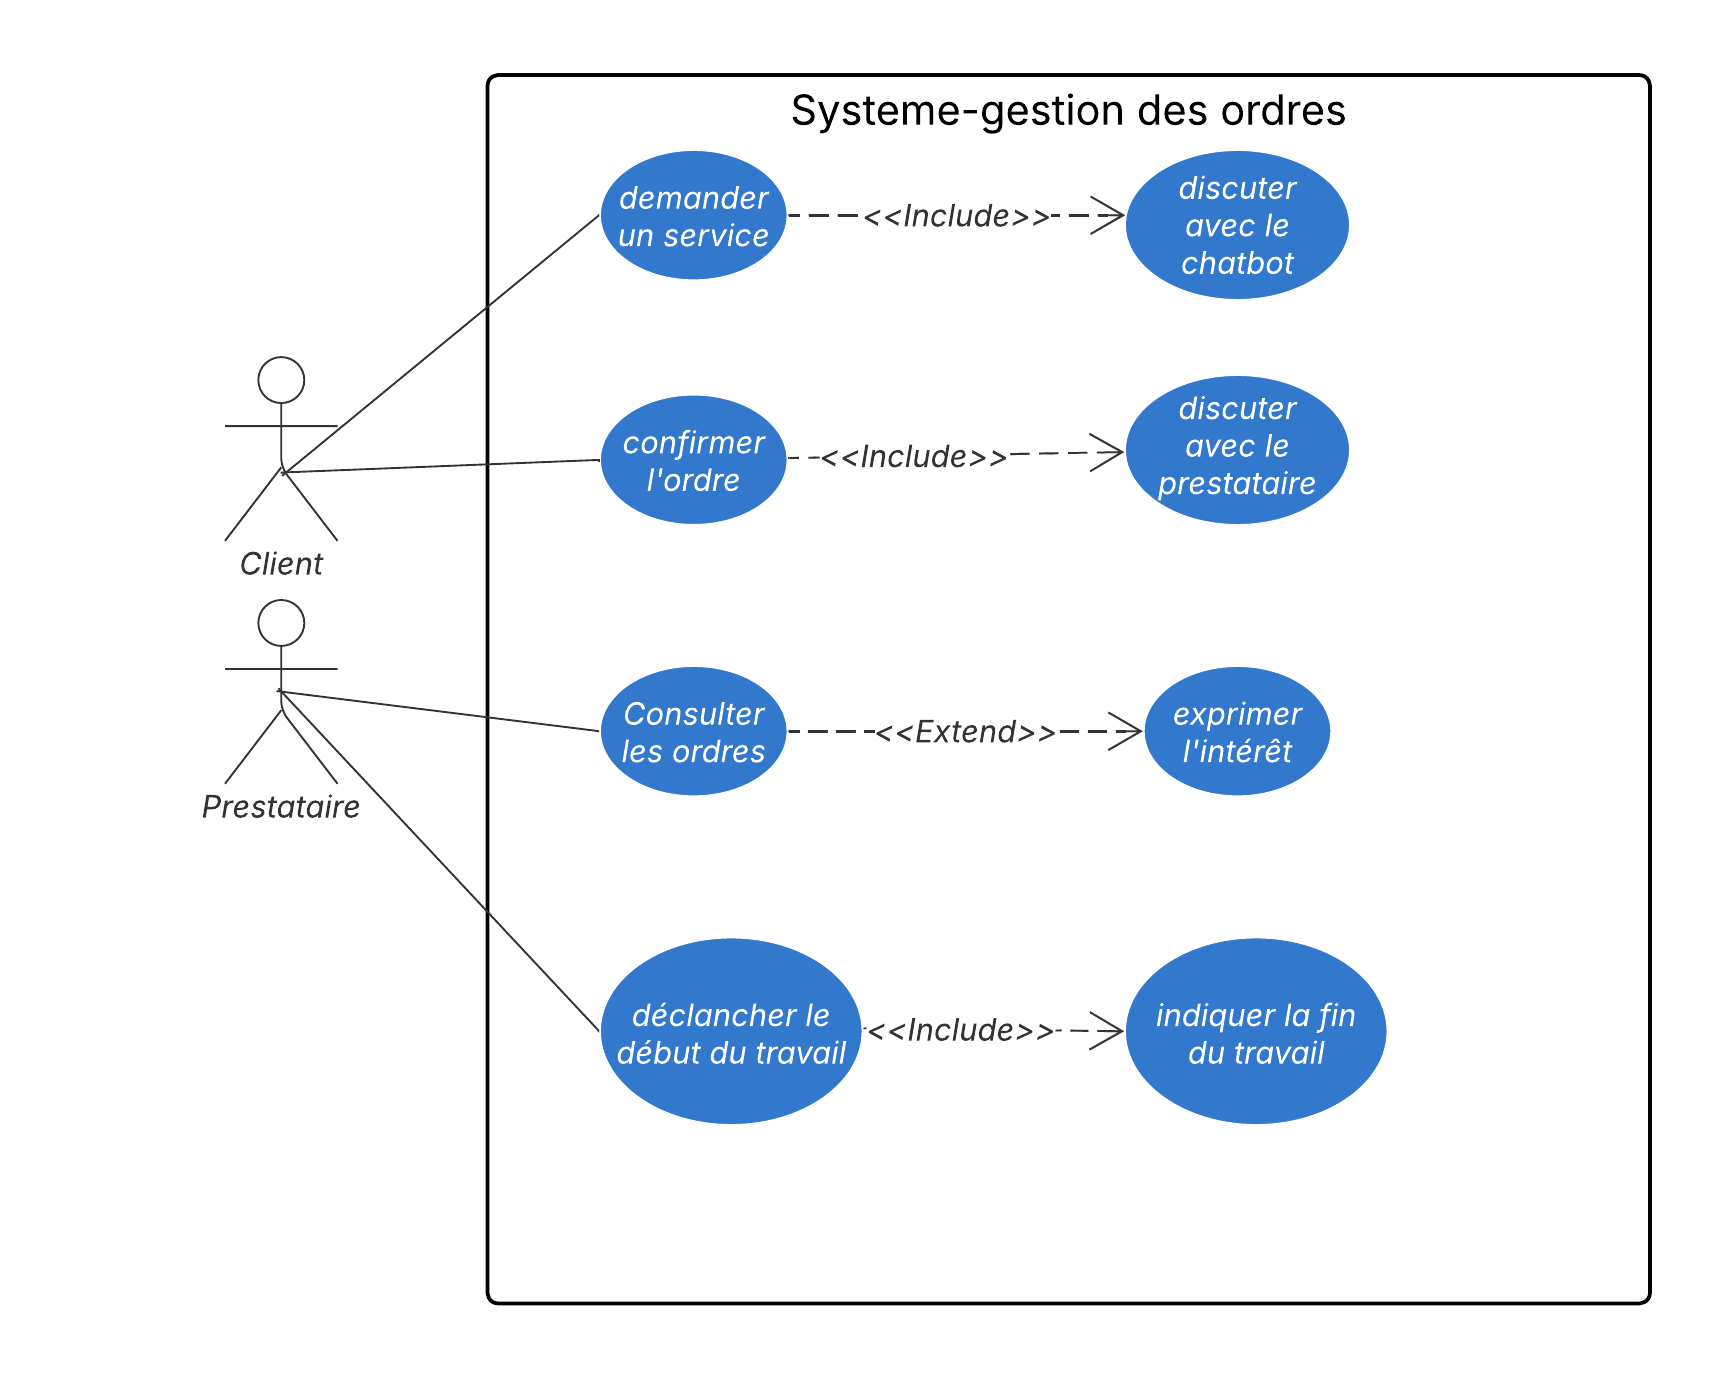
\includegraphics[width=0.85\linewidth]{figures/diagramme de cas d'utilisation gestion ordres.png}
\caption{Diagramme de cas d'utilisation raffiné – Gestion des ordres de mission}
\end{figure}

\textit{Ce diagramme illustre les interactions principales entre les acteurs (client et prestataire) et le système de gestion des ordres. Le client peut initier une demande de service, la confirmer, ou interagir avec le prestataire via un chatbot. Du côté du prestataire, celui-ci a la possibilité de consulter les ordres, exprimer son intérêt, déclencher le début d'une mission et signaler sa fin. Les cas d'utilisation inclus ou étendus montrent les dépendances fonctionnelles entre les actions.}


\section*{Diagrammes de séquence}
\subsection*{Diagramme de séquence – Consulter les ordres de mission disponibles}
\begin{figure}[H]
\centering
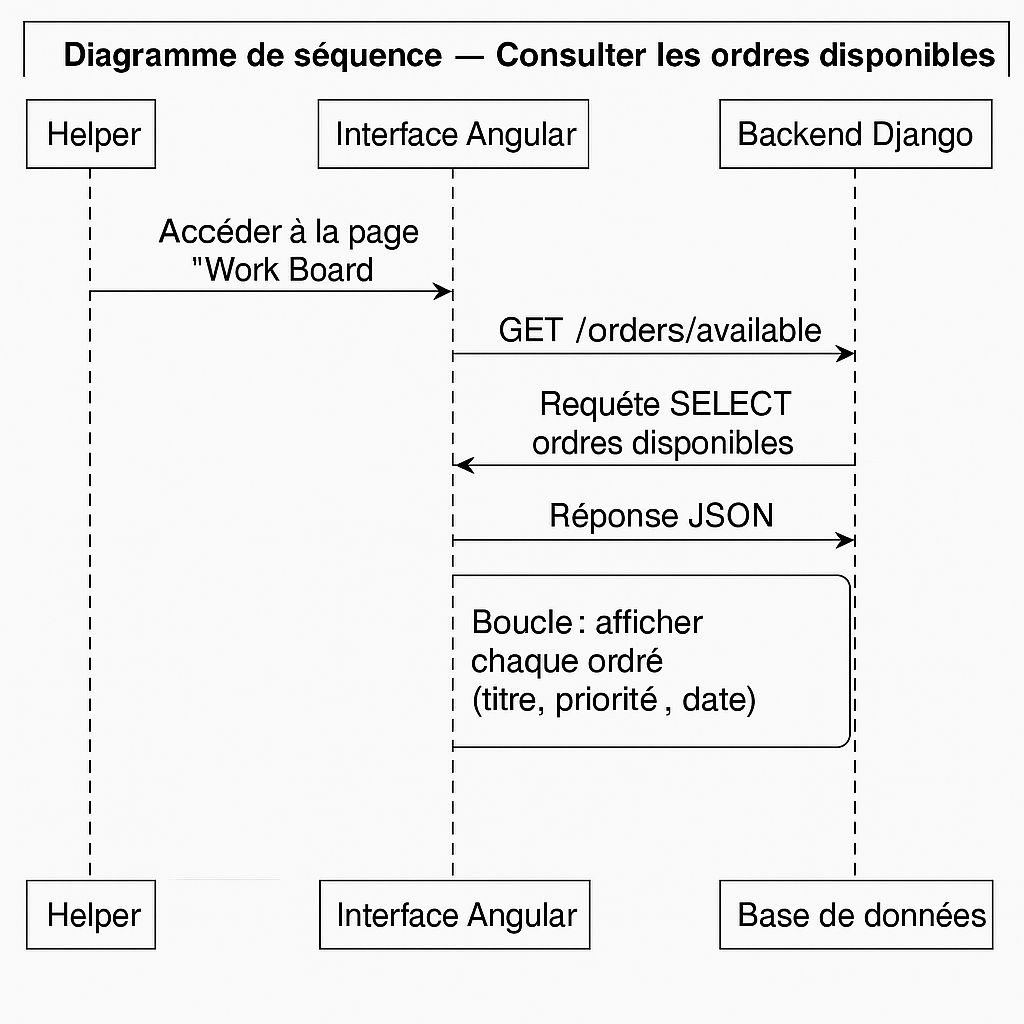
\includegraphics[width=0.85\linewidth]{figures/Diagramme de sequence cons ordres .png}
\caption{Consulter les ordres de mission disponibles}
\end{figure}

\textit{Ce diagramme de séquence décrit le processus de consultation des ordres de mission disponibles par un prestataire. Lorsque celui-ci accède à la page "Work Board" depuis l'interface Angular, une requête GET est envoyée au backend Django. Ce dernier interroge la base de données afin de récupérer les ordres disponibles. La réponse, au format JSON, est ensuite renvoyée à l'interface Angular, qui boucle sur chaque ordre pour les afficher avec leurs attributs tels que le titre, la priorité ou la date d'exécution.}


\subsection*{Diagramme de séquence – Exprimer l'intérêt pour un ordre}
\begin{figure}[H]
\centering
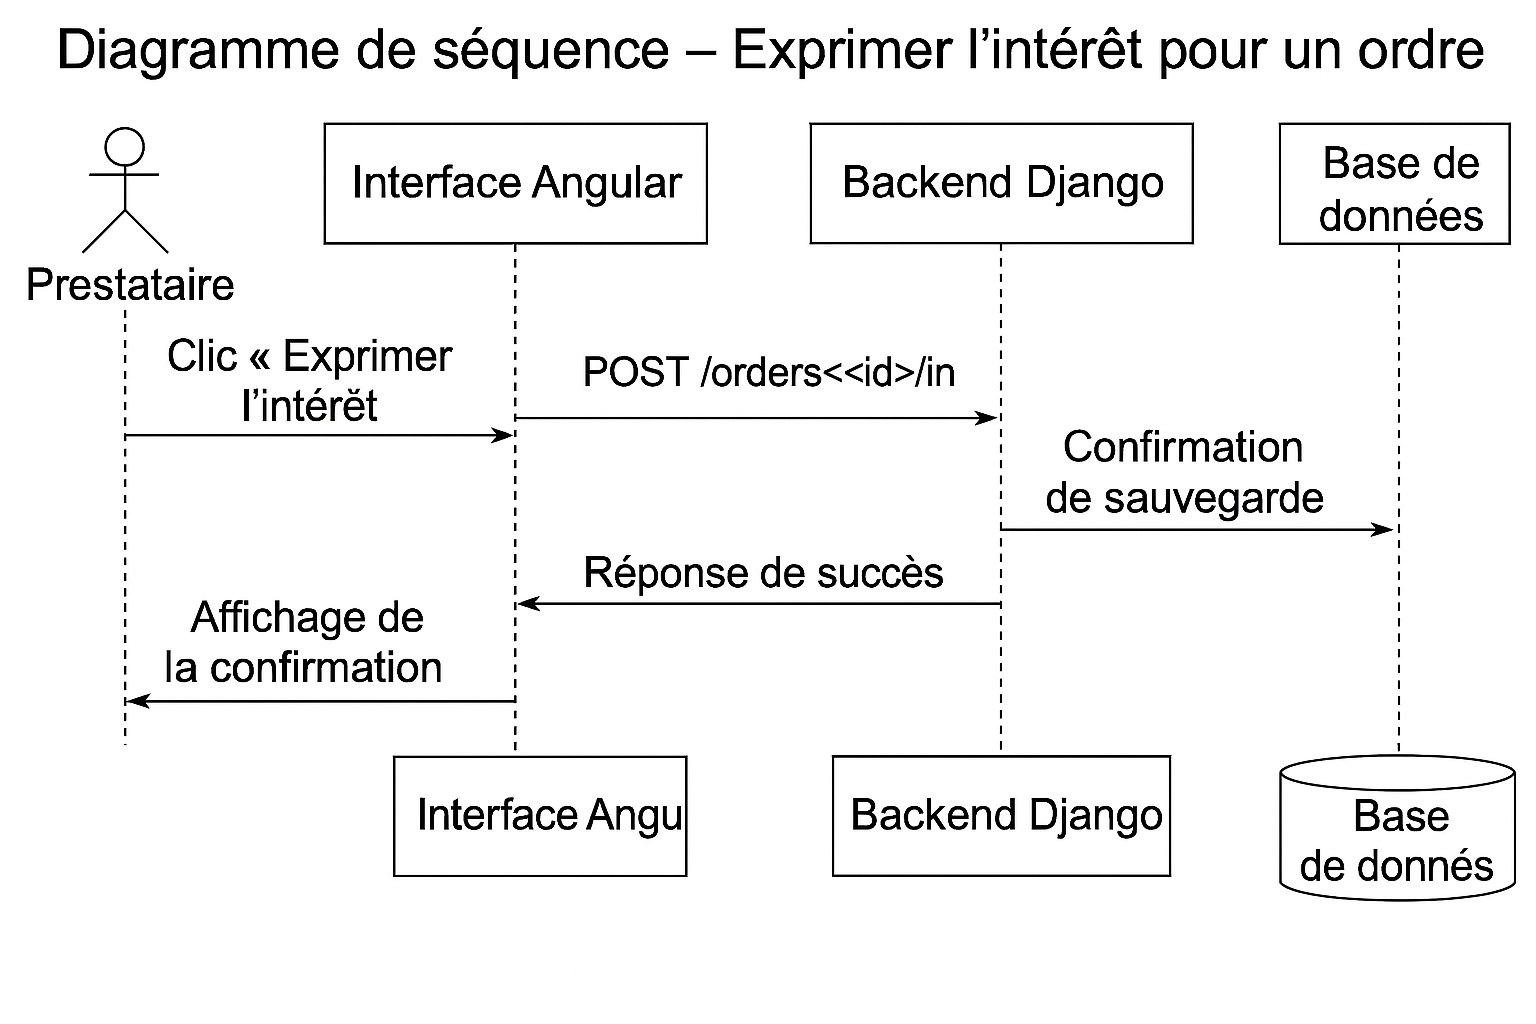
\includegraphics[width=0.85\linewidth]{figures/exprimer d'interet seq.png}
\caption{Exprimer l'intérêt pour un ordre}
\end{figure}

\textit{Ce diagramme de séquence présente les interactions déclenchées lorsqu’un prestataire exprime son intérêt pour un ordre spécifique. L’utilisateur clique sur le bouton “Exprimer l’intérêt” dans l’interface Angular. Cette action envoie une requête POST vers le backend Django via l’API REST. Le backend vérifie les paramètres, puis enregistre l’information dans la base de données. Une réponse de confirmation est ensuite renvoyée à l’interface, qui affiche un message visuel à l’utilisateur indiquant que sa demande a bien été prise en compte.}


\subsection*{Diagramme de séquence – Générer la facture après service}
\begin{figure}[H]
\centering
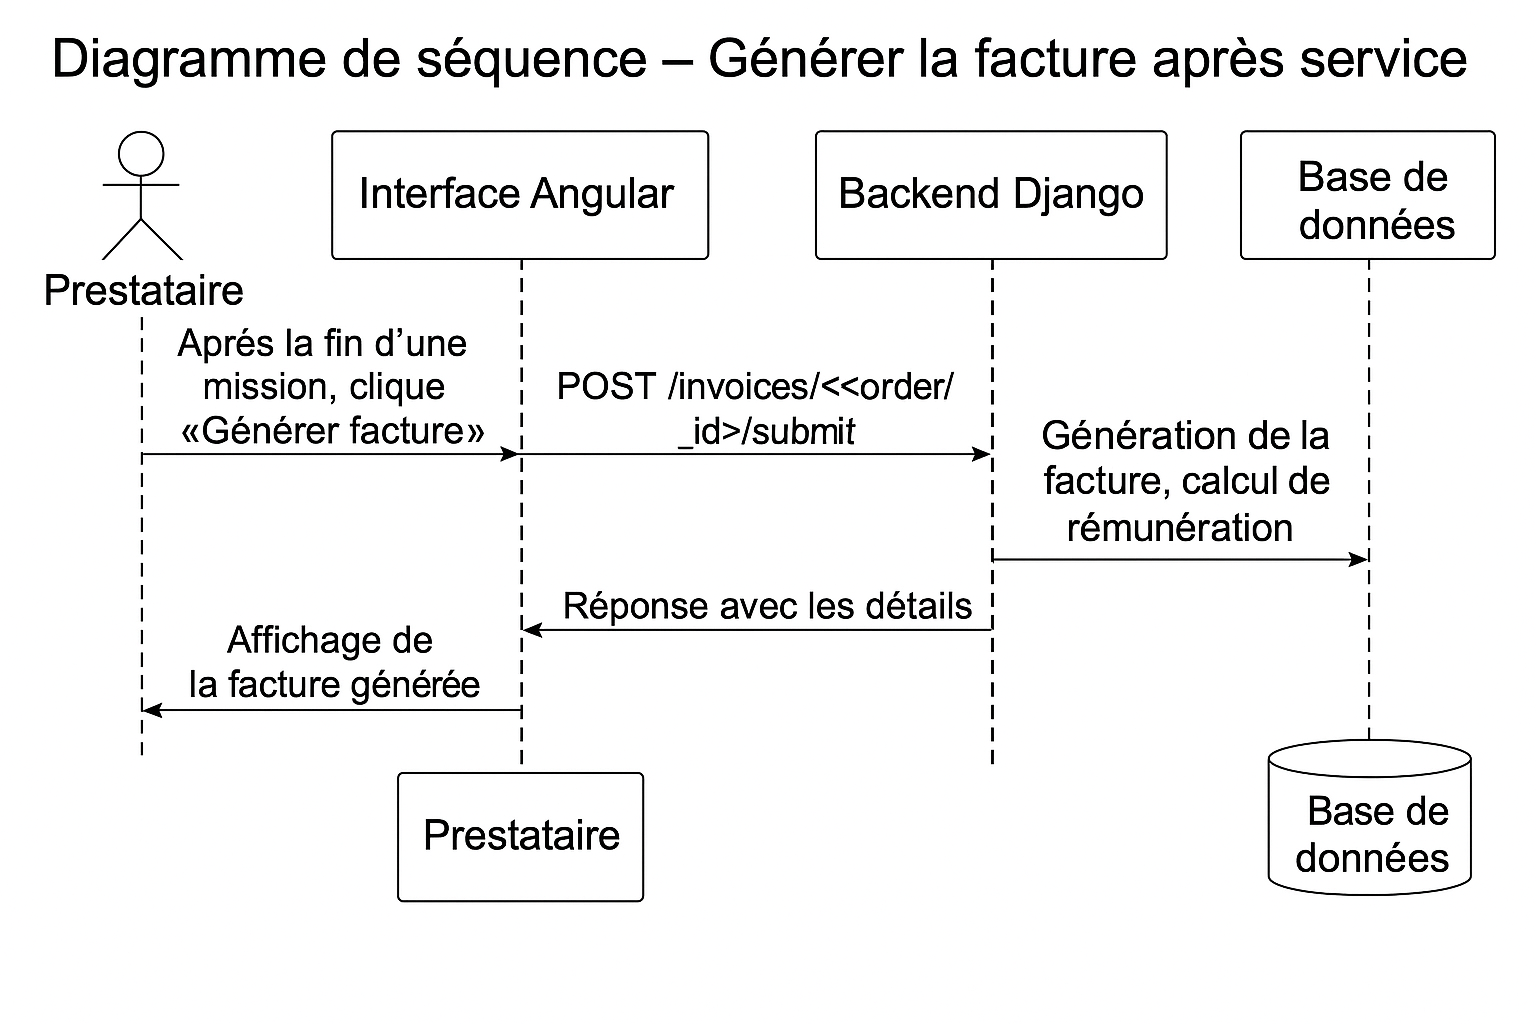
\includegraphics[width=0.85\linewidth]{figures/facture seq.png}
\caption{Générer la facture après service}
\end{figure}

\textit{Ce diagramme de séquence illustre le processus de génération d’une facture à la fin d’une mission. Une fois la mission terminée, le prestataire clique sur le bouton “Générer facture” dans l’interface Angular. Une requête POST est alors envoyée au backend Django, qui calcule le montant à facturer selon les données de la mission (durée, taux horaire, frais supplémentaires, etc.). La facture est ensuite enregistrée dans la base de données. Enfin, une réponse contenant les détails de la facture est renvoyée à l’interface, qui l’affiche à l’écran pour consultation.}


\subsection*{Diagramme de séquence – Suivre les missions confirmées}
\begin{figure}[H]
\centering
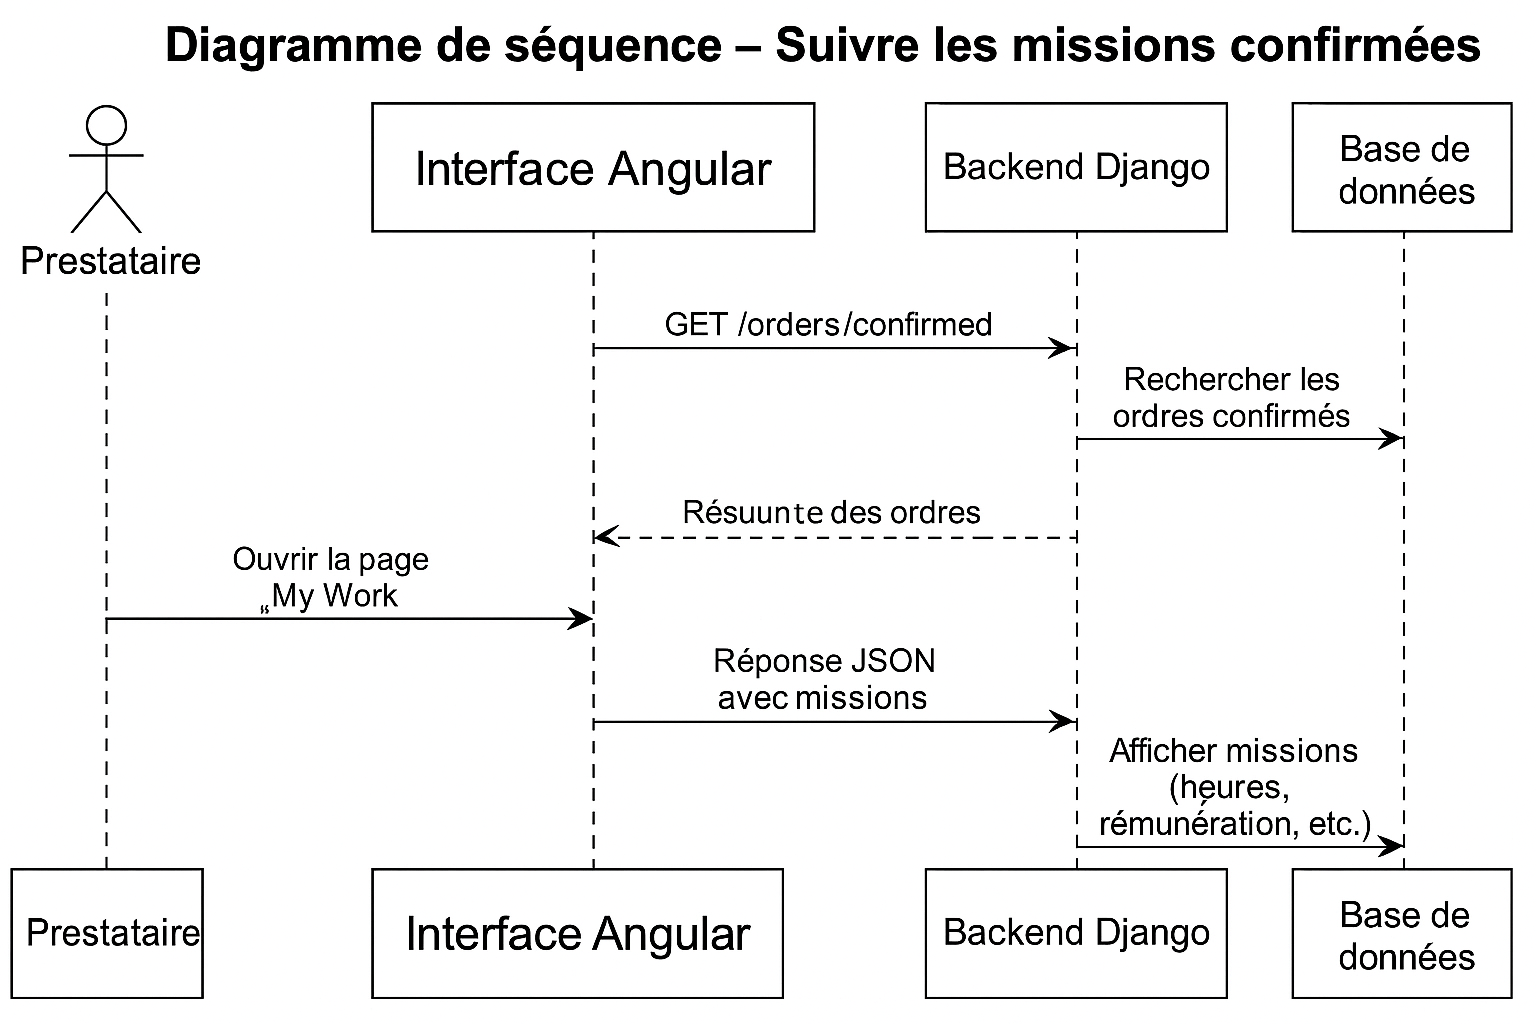
\includegraphics[width=0.85\linewidth]{figures/work seq.png}
\caption{Suivre les missions confirmées}
\end{figure}

\textit{Ce diagramme de séquence décrit le processus permettant à un prestataire de consulter les missions qui lui ont été officiellement attribuées. Lorsqu’il accède à la section “Mes missions” depuis l’interface Angular, une requête GET est envoyée au backend Django pour récupérer les ordres confirmés. Le backend interroge alors la base de données pour extraire les missions associées à l’utilisateur connecté. Une fois les données reçues, l’interface les affiche sous forme de cartes ou de tableau, avec les détails tels que la date, le client, la localisation et le statut.}


\section*{Diagrammes d'activité}
\subsubsection*{Diagramme d’activité – Expression d'intérêt pour une mission}
\begin{figure}[H]
\centering
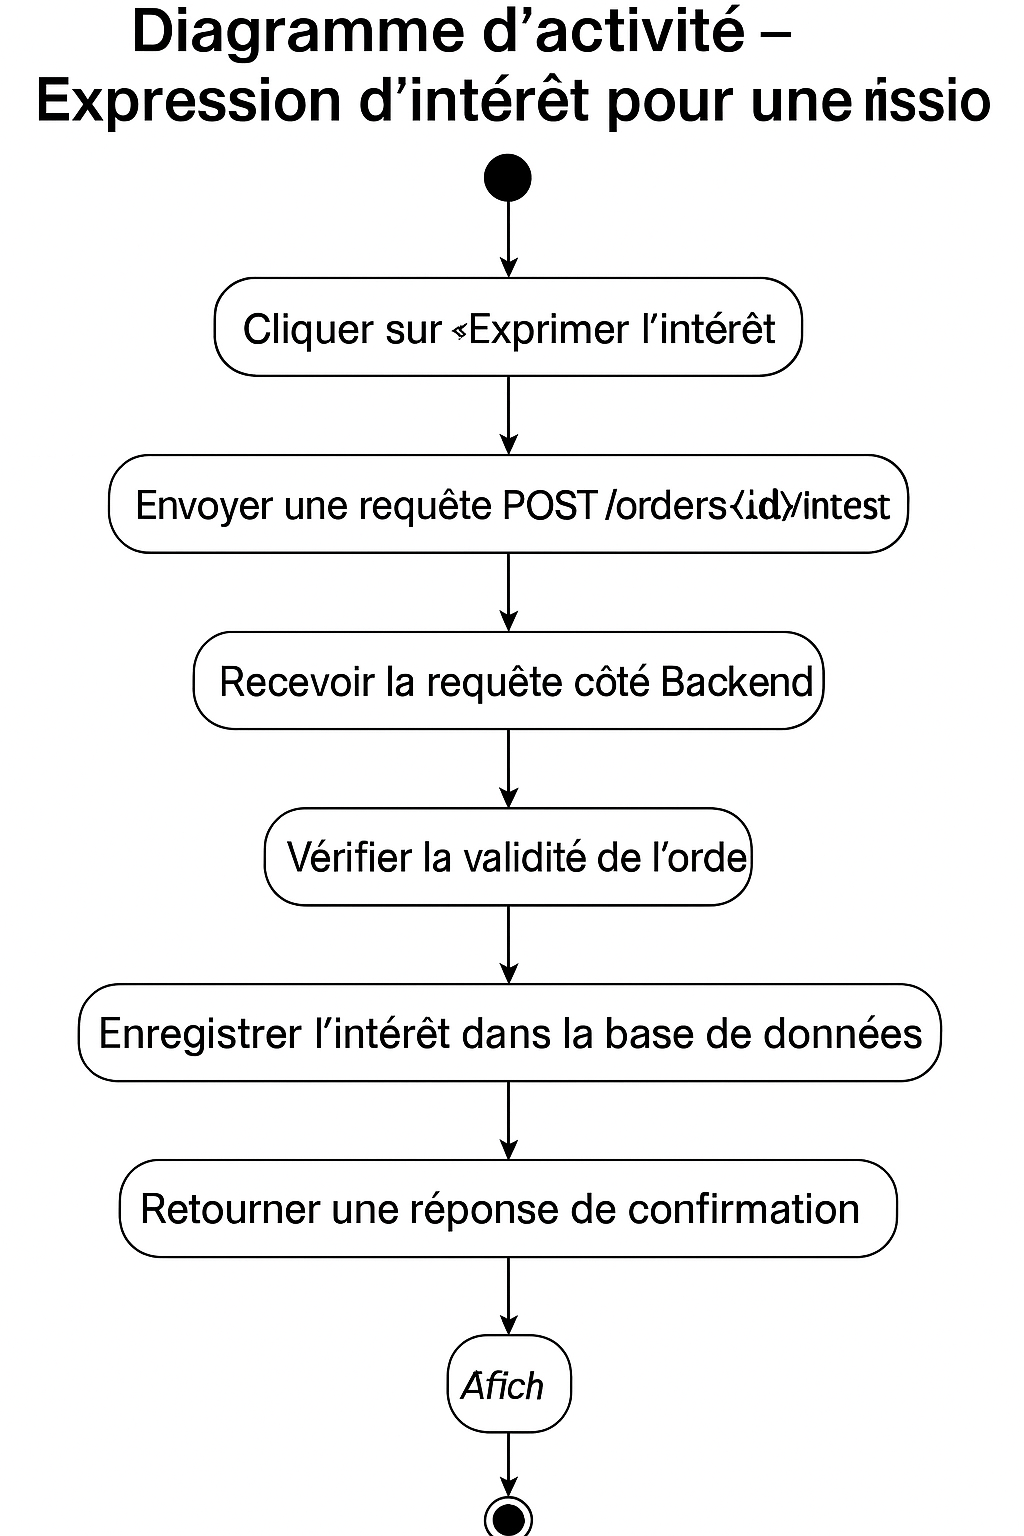
\includegraphics[width=0.85\linewidth]{figures/interet act.png}
\caption{Expression d'intérêt pour une mission}
\end{figure}

\textit{Ce diagramme d’activité illustre le déroulement des étapes permettant à un prestataire d’exprimer son intérêt pour un ordre de mission. L’activité commence par l’ouverture de la liste des ordres disponibles. Le prestataire sélectionne une mission, puis clique sur le bouton “Exprimer l’intérêt”. L’interface envoie ensuite une requête POST au serveur. Si la validation est réussie, l’intérêt est enregistré, et une confirmation est affichée à l’utilisateur. Le diagramme met également en évidence les décisions conditionnelles et les transitions logiques du flux.}

\subsection*{Diagramme d’activité – Consultation des ordres disponibles}
\begin{figure}[H]
\centering
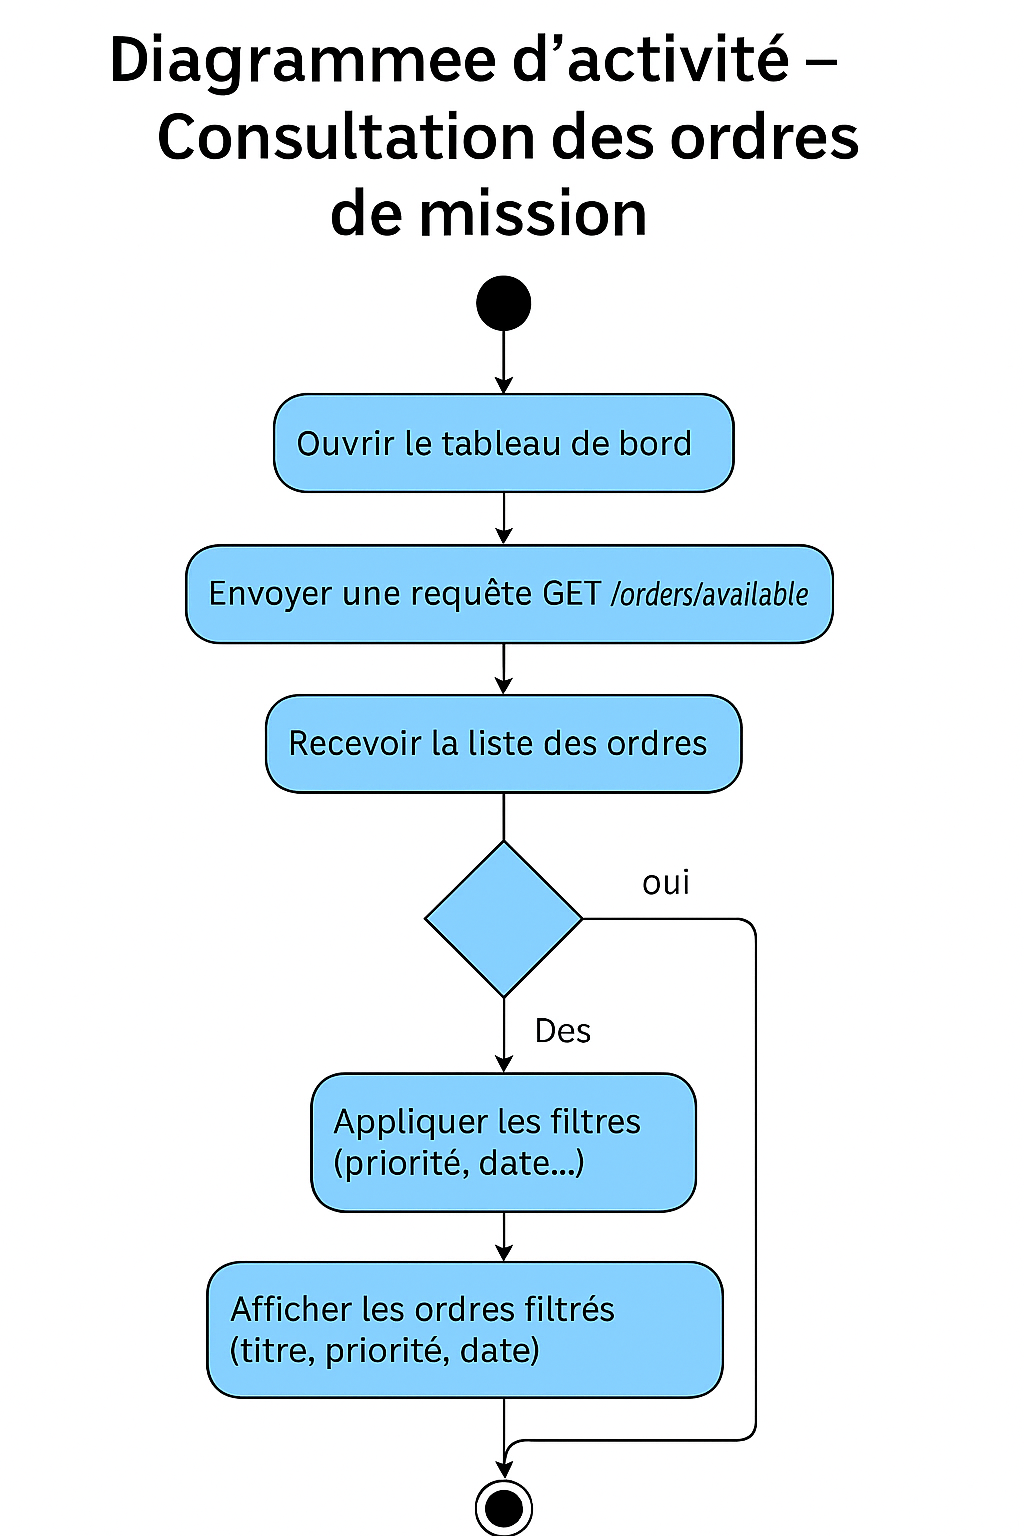
\includegraphics[width=0.85\linewidth]{figures/const ordres act.png}
\caption{Consultation des ordres disponibles}
\end{figure}

\textit{Ce diagramme d’activité détaille le processus permettant à un prestataire de consulter les ordres de mission disponibles. L’activité commence lorsque l’utilisateur accède au tableau de bord. L’interface déclenche une requête vers le backend pour récupérer les ordres. Après réception, les ordres sont filtrés selon des critères (priorité, localisation, etc.), puis affichés à l’écran. Le diagramme illustre les différentes étapes du traitement, y compris les décisions de filtrage, les actions d’affichage, et les éventuelles erreurs de chargement.}


\subsection*{Diagramme d’activité – Génération de la facture après mission}
\begin{figure}[H]
\centering
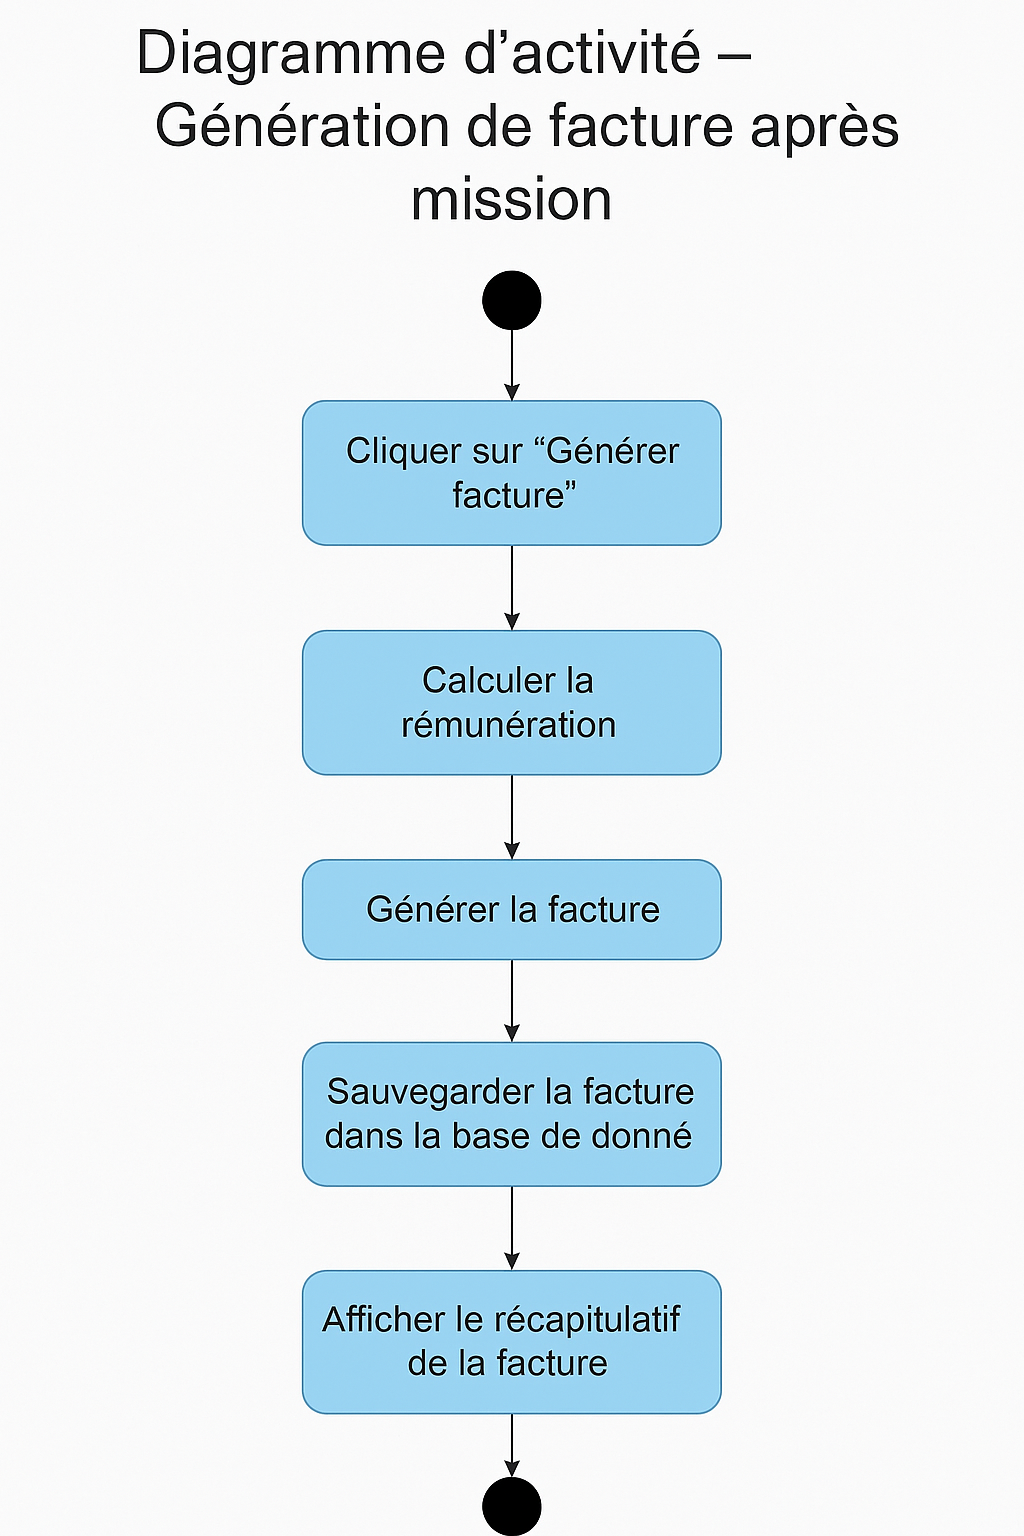
\includegraphics[width=0.85\linewidth]{figures/facture act.png}
\caption{Génération de la facture après mission}
\end{figure}

\textit{Ce diagramme d’activité décrit le processus déclenché par un prestataire pour générer une facture à la fin d’une mission. L’utilisateur démarre l’activité depuis l’interface en cliquant sur le bouton “Générer facture”. L’application vérifie d’abord si la mission est bien terminée. Si c’est le cas, une requête est envoyée au backend, qui calcule le montant à facturer à partir des données enregistrées (durée, taux horaire, frais, etc.). Une fois la facture créée, elle est sauvegardée, puis affichée à l’utilisateur.}


\subsection*{Diagramme d’activité – Suivi des missions confirmées}
\begin{figure}[H]
\centering
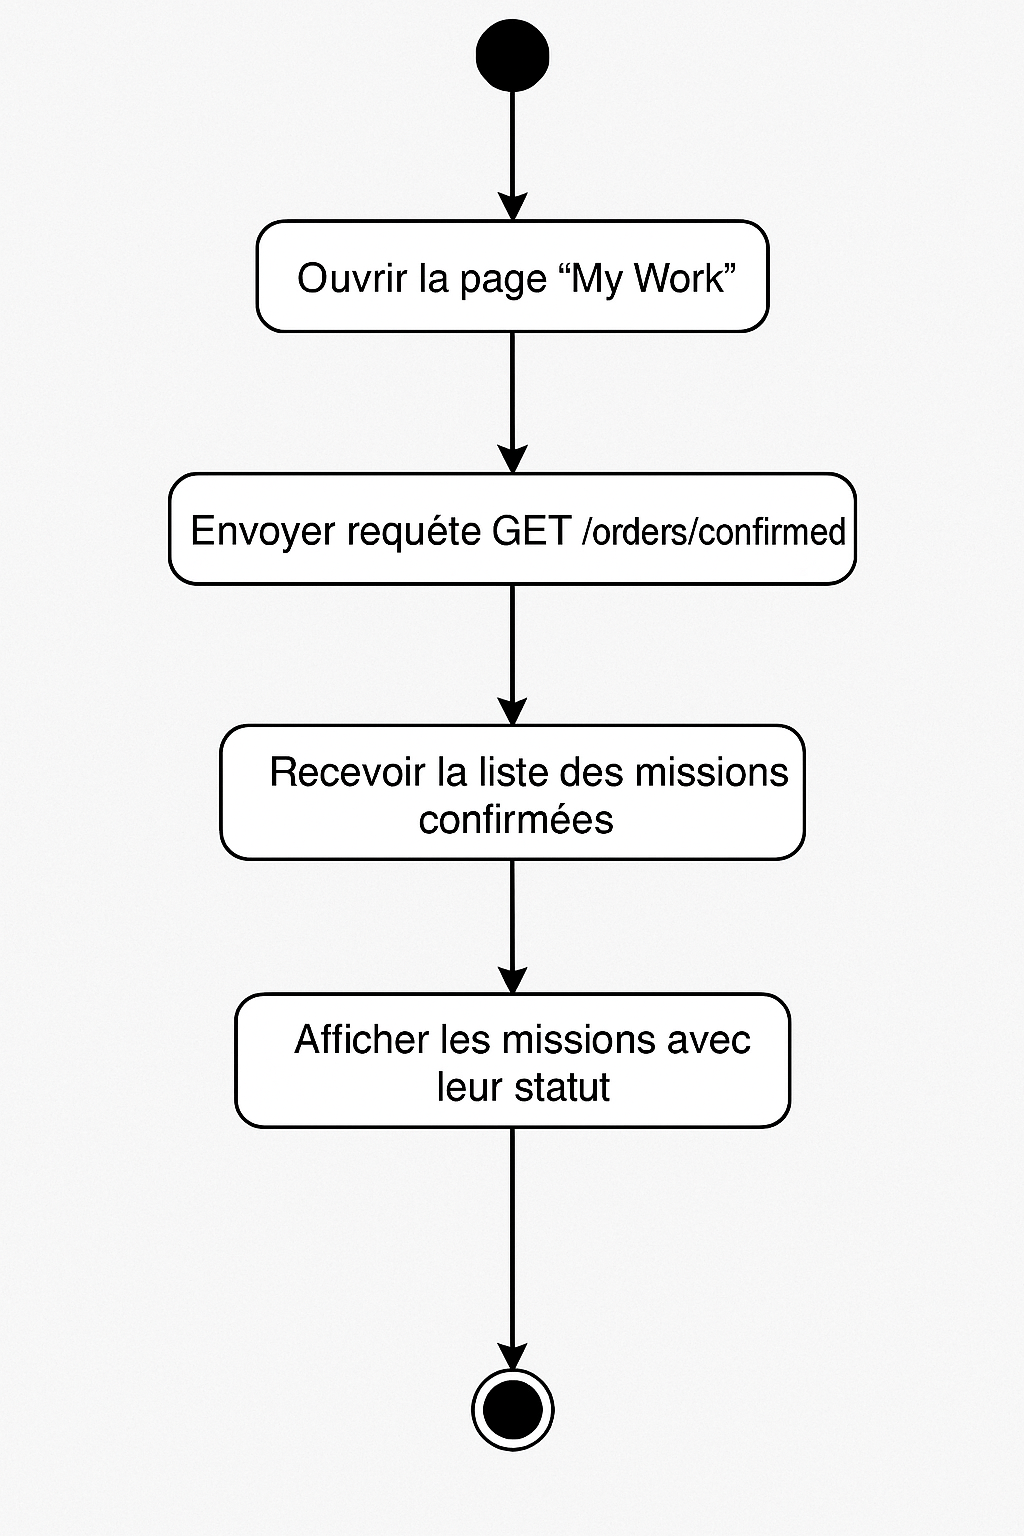
\includegraphics[width=0.85\linewidth]{figures/work act.png}
\caption{Suivi des missions confirmées}
\end{figure}

\textit{Ce diagramme d’activité décrit le processus permettant au prestataire de visualiser ses missions confirmées. Dès l’accès à la page “Mes missions”, une requête est envoyée au backend afin de récupérer les ordres de mission attribués. Les missions sont ensuite triées et affichées sous forme de calendrier ou de liste. Le prestataire peut consulter les détails de chaque mission, comme la date, l’heure, le client, ou encore le statut d’exécution. Ce diagramme met en évidence la logique conditionnelle et les étapes de récupération et d’affichage des données.}


\section*{Aperçu sur le code}
\subsection*{Aperçu sur le Backend}
\noindent
Cette capture représente un extrait du code backend développé avec Django. Elle concerne le modèle de données lié à la gestion des ordres de mission.

\begin{figure}[H]
\centering
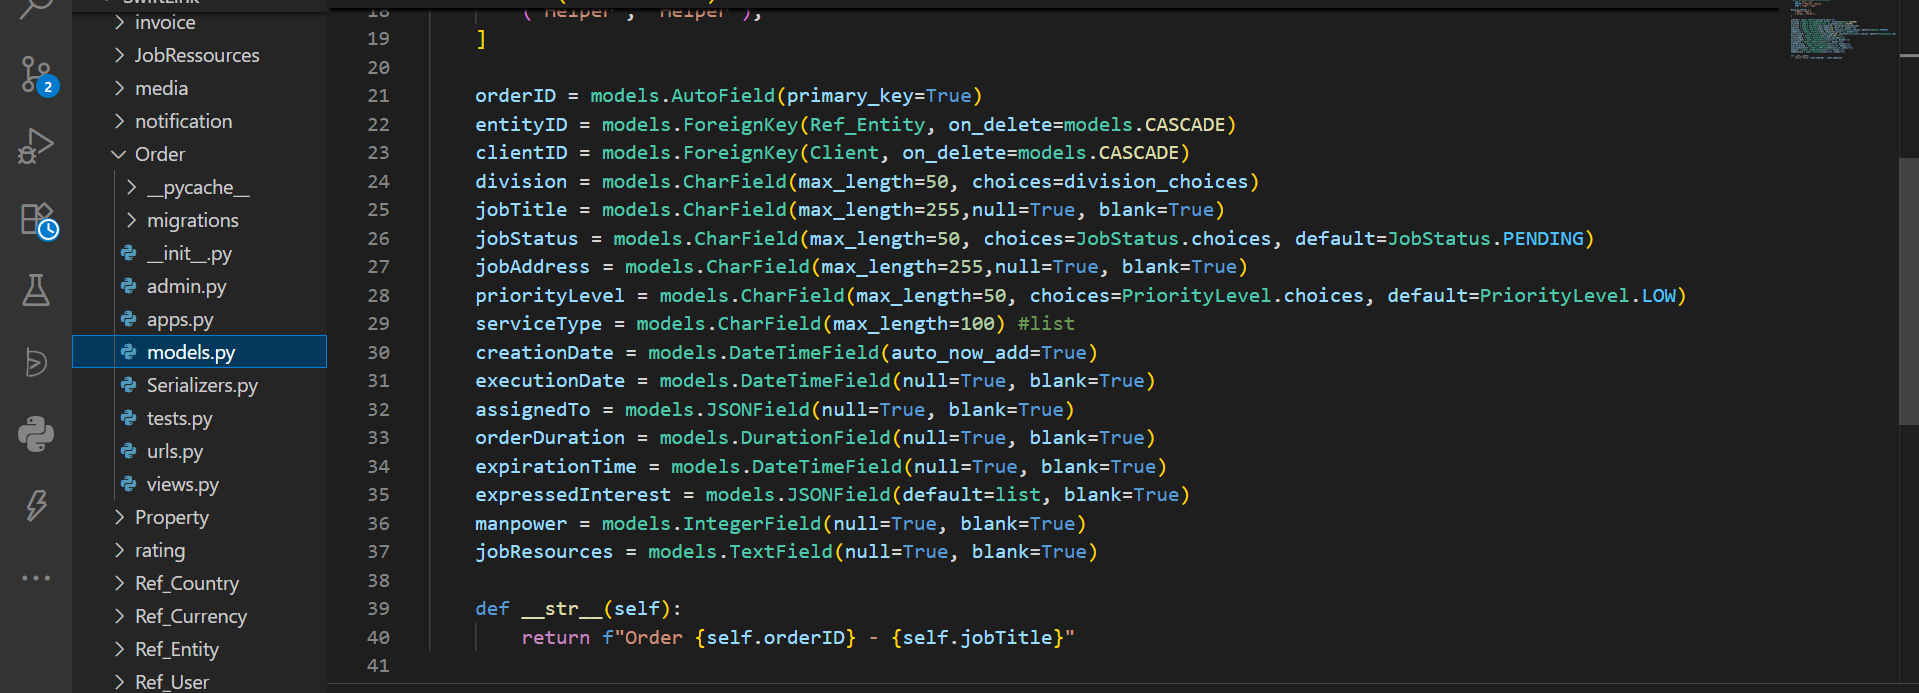
\includegraphics[width=0.85\linewidth]{figures/appercue code backend.png}
\caption*{\textit{Structure du modèle Django des ordres avec les champs associés. Le modèle définit notamment la relation avec le client, le prestataire, les statuts possibles, la priorité, et les métadonnées nécessaires à l’exécution et au suivi du service.}}
\end{figure}

\subsection*{Aperçu sur le frontend}
\noindent
Cette capture montre un extrait du composant Angular dédié à l’affichage des ordres de mission côté prestataire.

\begin{figure}[H]
\centering
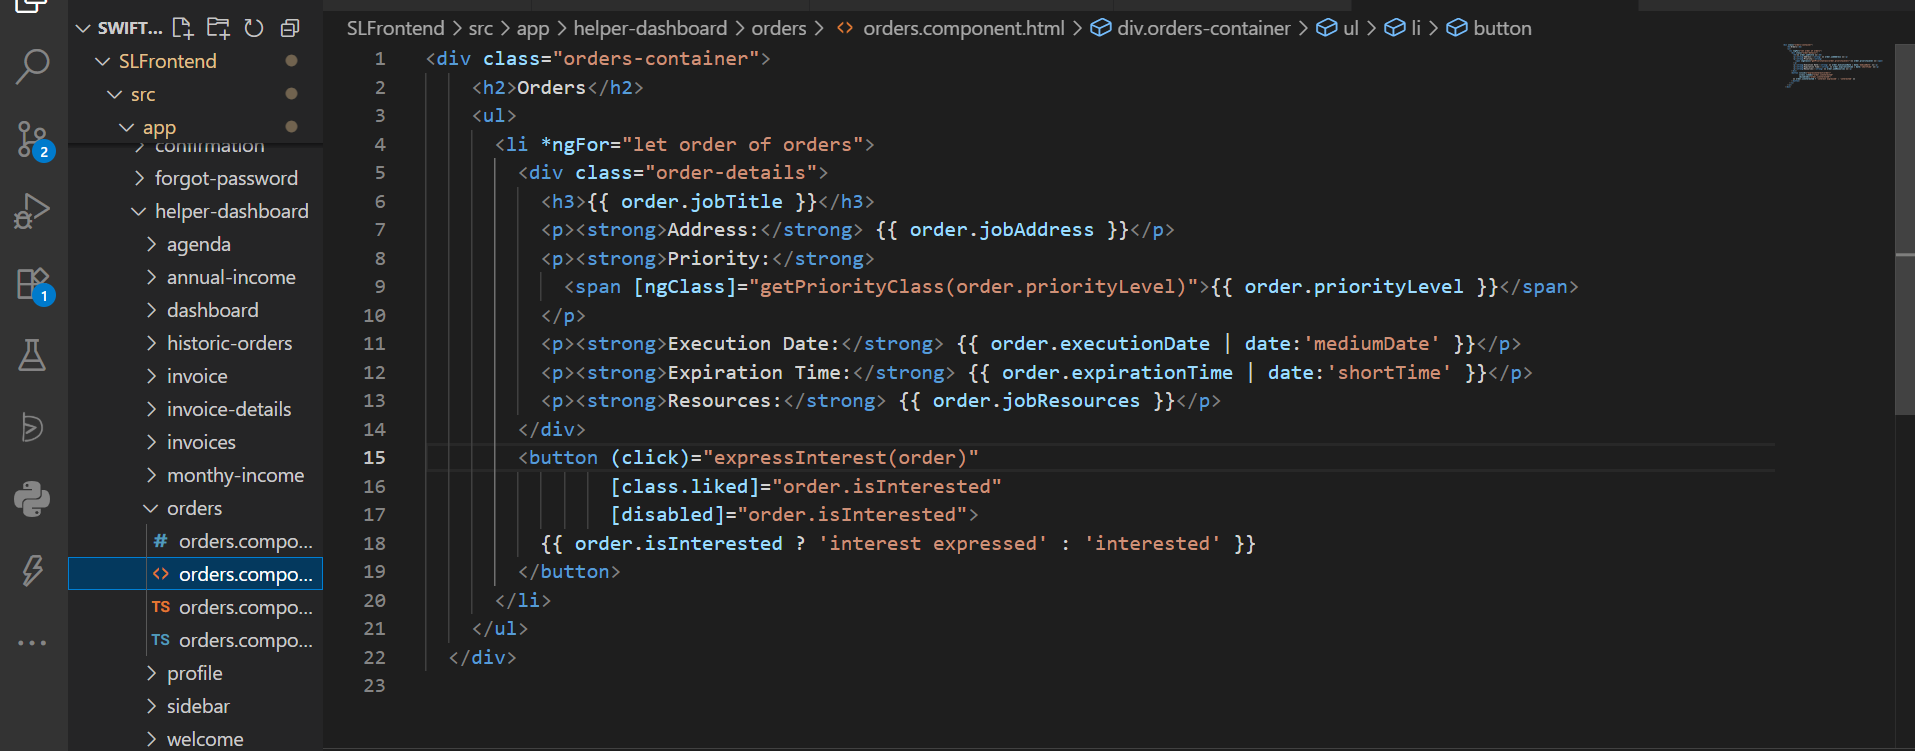
\includegraphics[width=0.85\linewidth]{figures/apercue code frontend.png}
\caption*{\textit{Composant Angular affichant les détails d'un ordre et le bouton d'intérêt. Ce composant utilise la liaison de données pour afficher dynamiquement les informations de l’ordre sélectionné (adresse, date, client) et propose un bouton interactif permettant au prestataire d’exprimer son intérêt.}}
\end{figure}
\section*{Conclusion}

Le Sprint 03 a permis de doter la plateforme d’un mécanisme structuré et automatisé de gestion des ordres de mission, élément central de l’interaction entre clients et prestataires. Grâce aux interfaces dédiées, les prestataires peuvent désormais consulter les missions disponibles, manifester leur intérêt, suivre les missions confirmées et générer des factures sans intervention manuelle.

La mise en place de cette logique métier a nécessité une coordination étroite entre les composants Angular (frontend) et Django (backend), notamment pour la gestion des statuts, des filtres, et des échanges de données en temps réel.

Ce sprint marque une étape clé dans le fonctionnement opérationnel de Swift Helpers, en assurant une continuité entre la demande client et la prestation réalisée, tout en posant les bases pour la supervision et l’analyse des performances dans les sprints suivants.


